%%%%%%%%%%%%%%%%%%%%%%%%%%%%%%%%%%%%%%%%%%%%%%%%%%%%%%%%%%%%%%%%%%%%%%%%%%%%%
% Chapter 7: Presupuesto
%%%%%%%%%%%%%%%%%%%%%%%%%%%%%%%%%%%%%%%%%%%%%%%%%%%%%%%%%%%%%%%%%%%%%%%%%%%%%%%

%++++++++++++++++++++++++++++++++++++++++++++++++++++++++++++++++++++++++++++++


La siguiente tabla de la Figura \ref{fig:presupuesto} nos indica cuantas horas de trabajo e investigación abarcó cada características o funcionalidad de la aplicación, al igual que 
el número total de horas (346 horas) que duró la elaboración del proyecto incluyendo ambas características. \\

\begin{figure}[H]
\begin{center}
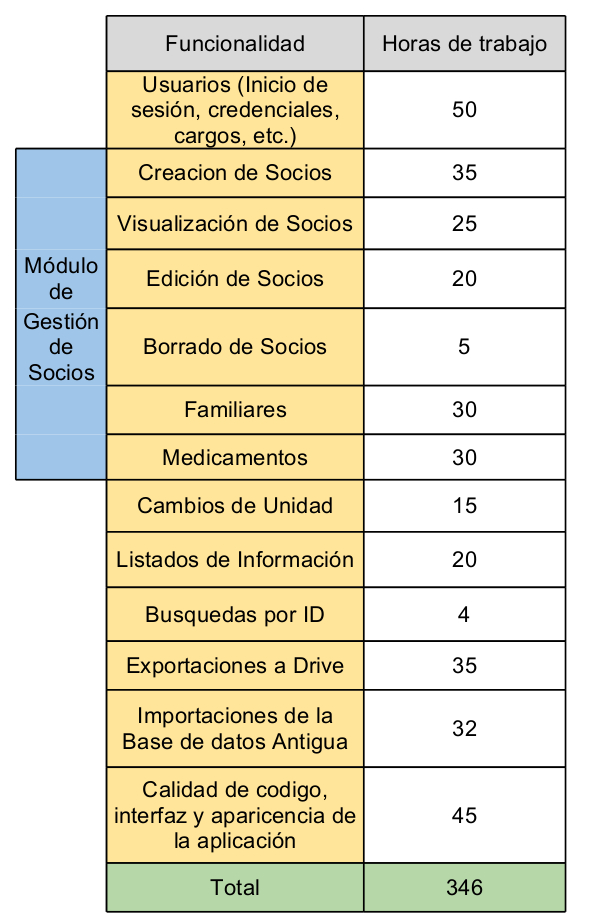
\includegraphics[width=0.65\textwidth]{images/presupuesto.jpg}
\caption{Números de horas totales y de desarrollo que se llevaron a cabo en el proyecto}
\label{fig:presupuesto}
\end{center}
\end{figure}

\newpage

Por otro lado, destacamos el porcentaje de investigación que tuvo cada funcionalidad, de esta manera podemos ver que funcionalidad fue más complicada de
desarrollar según su porcentaje de investigación. Y para finalizar se descontaron estas horas de investigación para obtener el número neto de horas de desarrollo de cada funcionalidad, cuya suma sera el 
total de horas exclusivas de desarrollo, que son las horas que se le facturaran al cliente (166,4 horas).\\


Dicho esto la tarifa por de desarrollo establecida en este proyecto es de \textbf{12 euros} la hora.\\

\bigskip

Por tanto la aplicación \textbf{GScout} tendrá un precio de: {\Huge \textbf{1996,90 euros}}\\


